\section{The \textit{Food Products} Trade Network}

% - Food network abbastanza interessante perchè aveva size grossa, facilmente interpretabile
The market of \textit{Food Products}\footnote{
    From the EU Economic Activity Classification:
    "This division includes: a variety of products that are the effect of farming, forestry, hunting and fishing, such as meat, fish, fruits and vegetables, fats and oils, dairy products, grain mill products, animal feeds, and other food products intended for humans or animals; semifinished products that are not directly food products; by-products of different value in use (e.g. the hides, oil-cake from the production of vegetable oils); treatment of slaughterhouse waste/waste seized at slaughterhouses/for the production of animal feed."\cite{eurostat2022website}
} is particularly interesting since it is one of the biggest in terms of amount of money exchanged. Moreover, its relationships may be easier to interpret, as they are strongly dictated by the geographical position, soil and climate conditions of countries, that are the main reason why some territories need to import many goods if they want to guarantee diversification in nutrition. Global food trade is of crucial importance for countries since it guarantees food security and availability. Studying the structure of this network allows understanding its vulnerability in terms of food security. Indeed, the interdependencies in food supply, which one can study analytically from trade data, can expose countries to supply risks, especially in periods of global stress, political instability or natural disasters \cite{wang2021evolution}. I will show how, using the method described in previous chapters, one is able to get an understanding of the dynamics of this network. With the data at the hand, the first thing one can do is to look at the graph metrics for this category and how they evolved over time, which provides a first impression of the evolution of the market. Figure \ref{fig:foodmetrics} shows four metrics as time series: size (sum of the weights), average degree, median page rank and average clustering coefficient. We can have a look at the time series to spot trends and variations that can be linked to the latest historical events. Indeed, in the upper left box, we can easily spot the huge drops in the size of the graph that happened during the 2008 financial crisis and the COVID crisis. 
Moreover, regarding 2020, we can see in the two plots on the right the effect of closing the borders to contain the pandemic: the average degree had an important drop since countries truncated or reduced a significant number of exchanges. This is an evidence of the contraction in food trade caused by the sudden outbreak of COVID in 2020, when, for example, some big exporters, suspended or banned grain exports.
At the same time, the steep increase in clustering can be attributed to it being inversely correlated with the average degree: when a node has fewer neighbors the denominator of Equation \ref{eq:clustering} decreases, and so the clustering coefficient goes up, even though the network as a whole may be less connected.
Lastly, in the bottom right plot we see the median page rank among nodes, and we can observe that it used to have a positive trend until 2013, but since then it had started to go down, even more so during COVID. This could be a signal of the market going from a slightly more centralized structure to having more producers and exporters.

\begin{figure}[H]
    \centering
    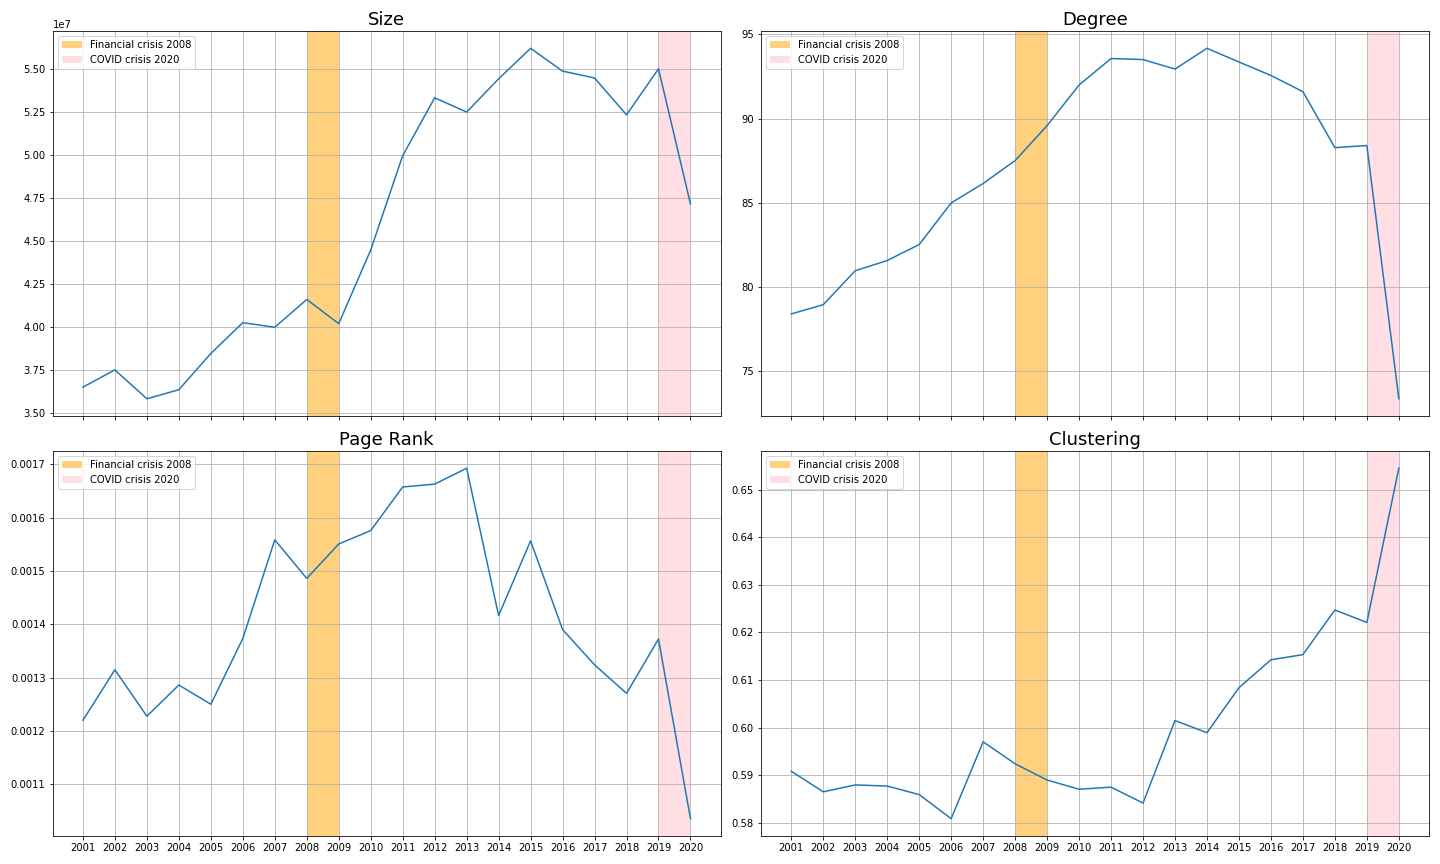
\includegraphics[width=\textwidth]{pics/full_p10_metric_ts.png}
    \caption{Food Metrics TODO}
    \label{fig:foodmetrics}
\end{figure}

\subsubsection*{Degree distribution}

Moving on with the analysis of the trade networks of the Food Products category, one can study the properties of the degree distribution of the graphs over time. As mentioned in Section \ref{sec:4powerlaw}, we can try to verify whether the networks show features of the scale-free property, that is whether there are just a few countries with a high number of trade flows. The procedure to check this is to fit a power law distribution $\alpha k^{-\gamma}$ on the degree distribution (or equivalently fit a simple linear regression on the log-log plot of the distribution) and check how well it fits. I have reported the results in Figure \ref{fig:fooddegree}. The four plots correspond to the four types of degree distribution that I can construct on a directed weighted graph, using in/out, weighted/unweighted degree. In each of these plots, it is reported in blue the power law exponent $\gamma$ for each year in my dataset, and in orange the Mean Absolute Percentage Error\footnote{
    $\text{MAPE}(y, \hat{y}) = \frac{1}{n_{\text{samples}}} \sum_{i=0}^{n_{\text{samples}}-1} \frac{{}\left| y_i - \hat{y}_i \right|}{\max(\epsilon, \left| y_i \right|)}$
} of the linear regression fit on the log-log plot. The MAPE should give us an idea on how well the power law is fit on the distribution: for example, we see that over all the years the fit for the \textit{in weight degree} is better than the one for the \textit{out weight degree}, meaning that there are just a few countries that import high amounts of goods per 1000 inhabitants, while the major exporters are not just a few. Considering instead $\gamma$, we see that the fit on the \textit{in degree} yields a generally lower exponent than the \textit{in weight degree}, meaning that in the former case the hyperbole is less steep than in the latter. 
\begin{figure}
    \centering
    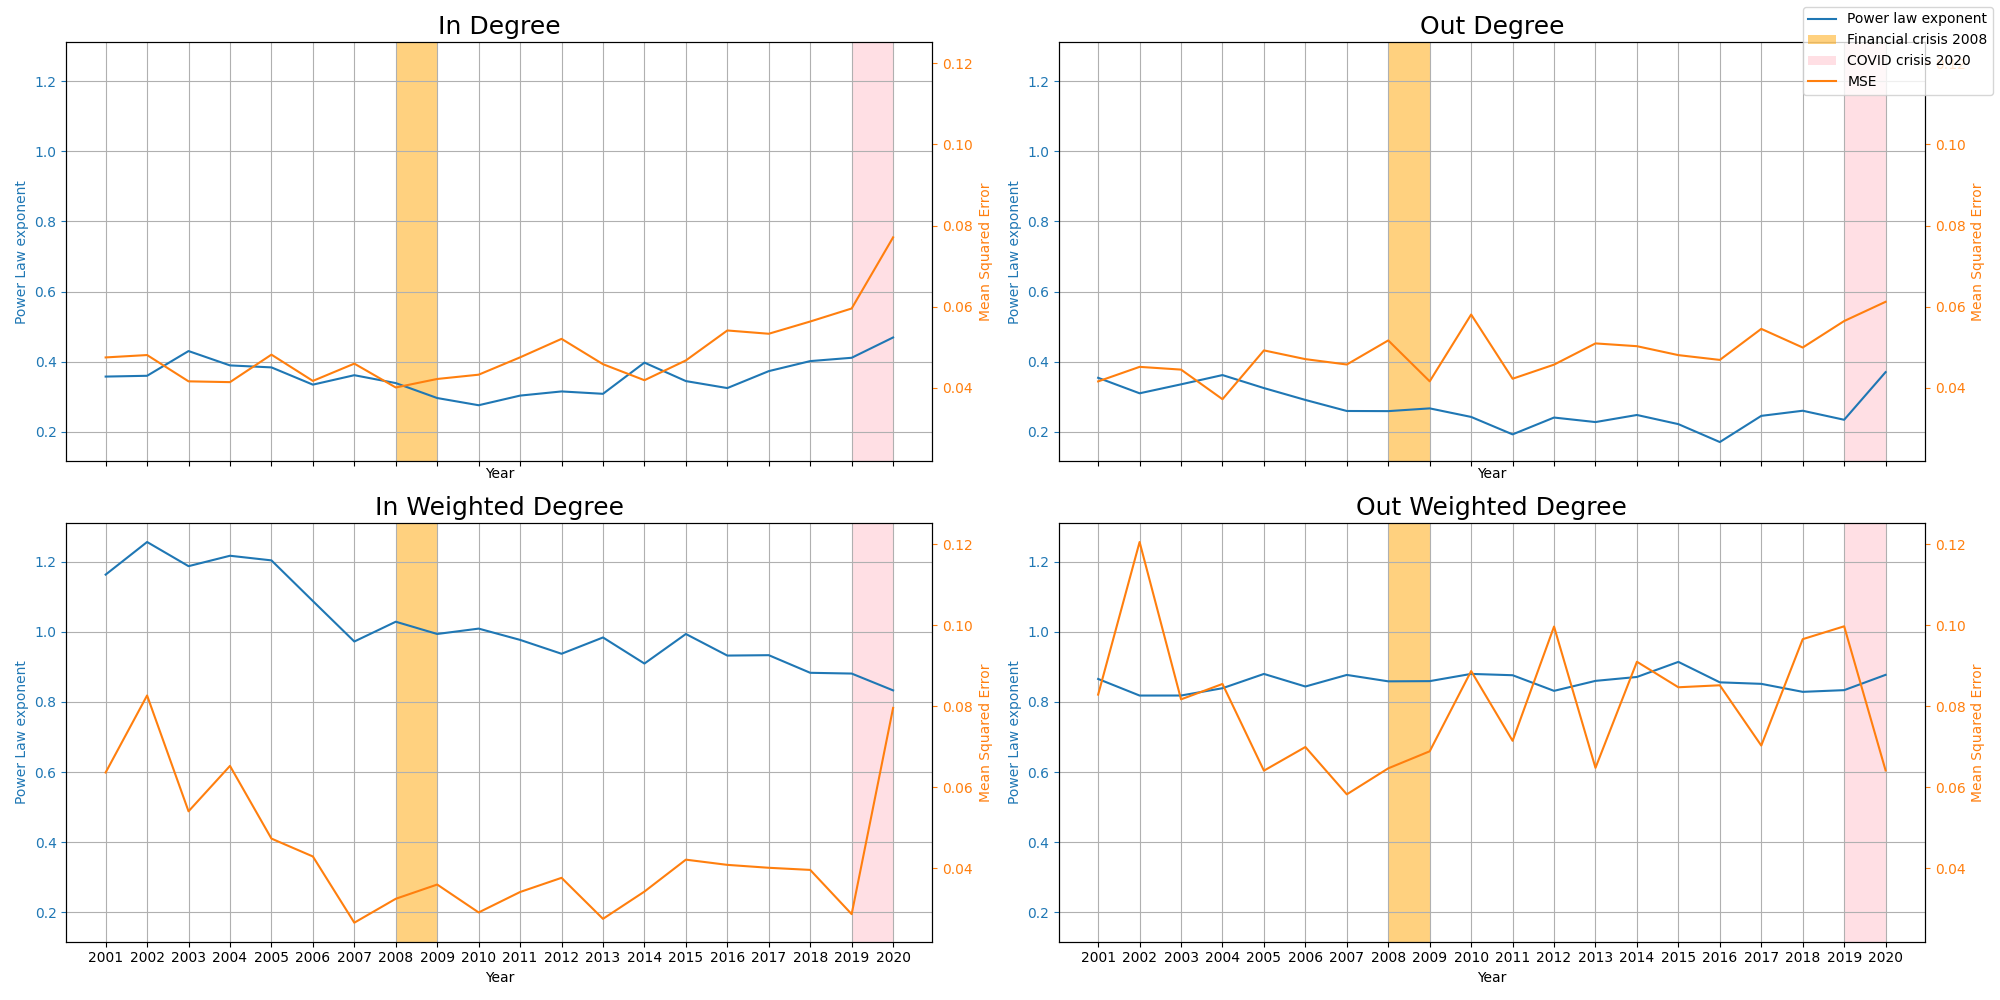
\includegraphics[width=\textwidth]{pics/ts_p10.png}
    \caption{Power law exponents over time of four degree distributions in the Food Products networks.}
    \label{fig:fooddegree}
\end{figure}
To better visualize this, let me choose a suitable year from the time series, for example 2010 which has a lower MSE, and let me plot the degree distribution of that year with its corresponding power law fit. This is shown in Figure \ref{fig:plfood} for the \textit{in degree} and Figure \ref{fig:plfoodw} for the \textit{in weight degree}. In each of these figures we see on the left the degree distribution as the blue dots, while the red curve is the fitted power law; on the right instead we have the same plot but with log-log axis, where the red curve becomes a straight line.
It is quite evident from these pictures that the distribution for the unweighted \textit{in degree} doesn't follow a power law distribution (hence the poor fit) and thus we conclude that this kind of unweighted network is not scale-free. When we look instead at the distribution of the \textit{in-strength}, we observe a better fit: this means that in the trade network for Food Products a high number of countries imports small quantities of goods relatively to their population, while instead a smaller portion of countries are less self-sufficient, and thus they have bigger imports. In short, this is not the case of a few countries occupying a large number of trade flows, but of just a few countries importing a high share of the traded goods.

\begin{figure}
    \centering
    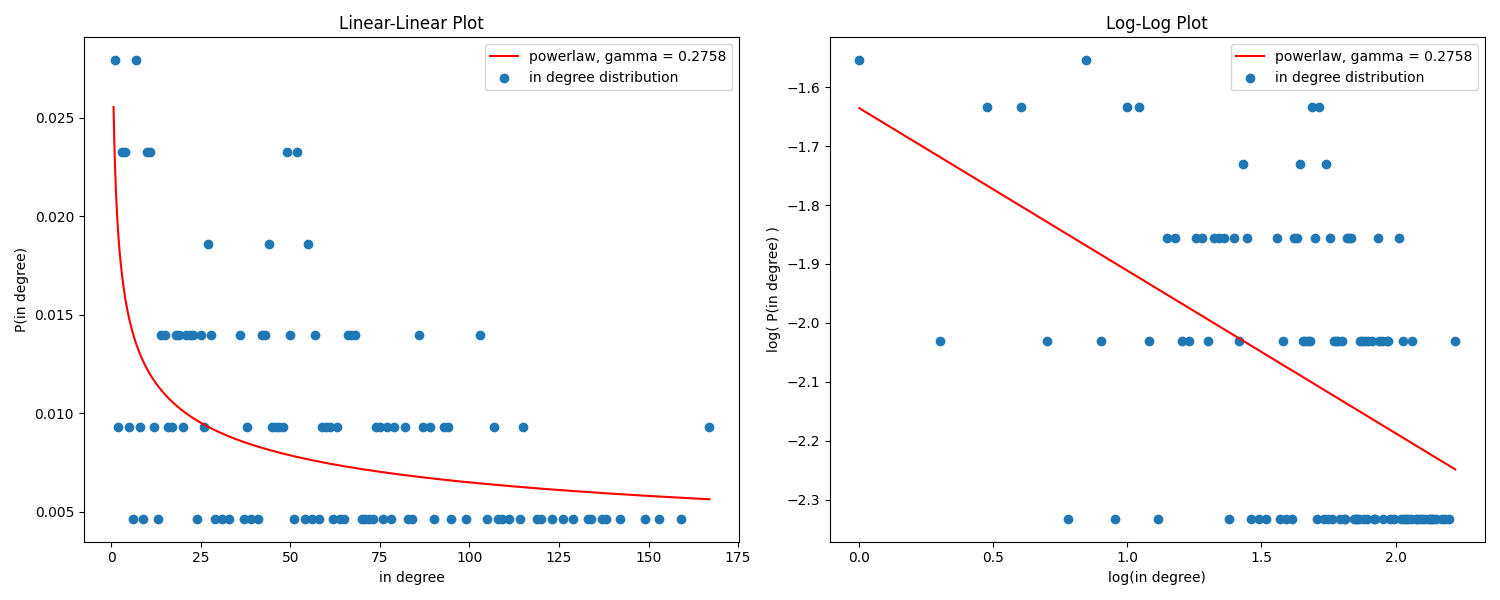
\includegraphics[width=\textwidth]{pics/powerlaw_in_degree_p10_y2010.png}
    \caption{Food Products trade network's degree distribution of the \textit{in degree} in 2010, with power law fit.}
    \label{fig:plfood}
\end{figure}

\begin{figure}
    \centering
    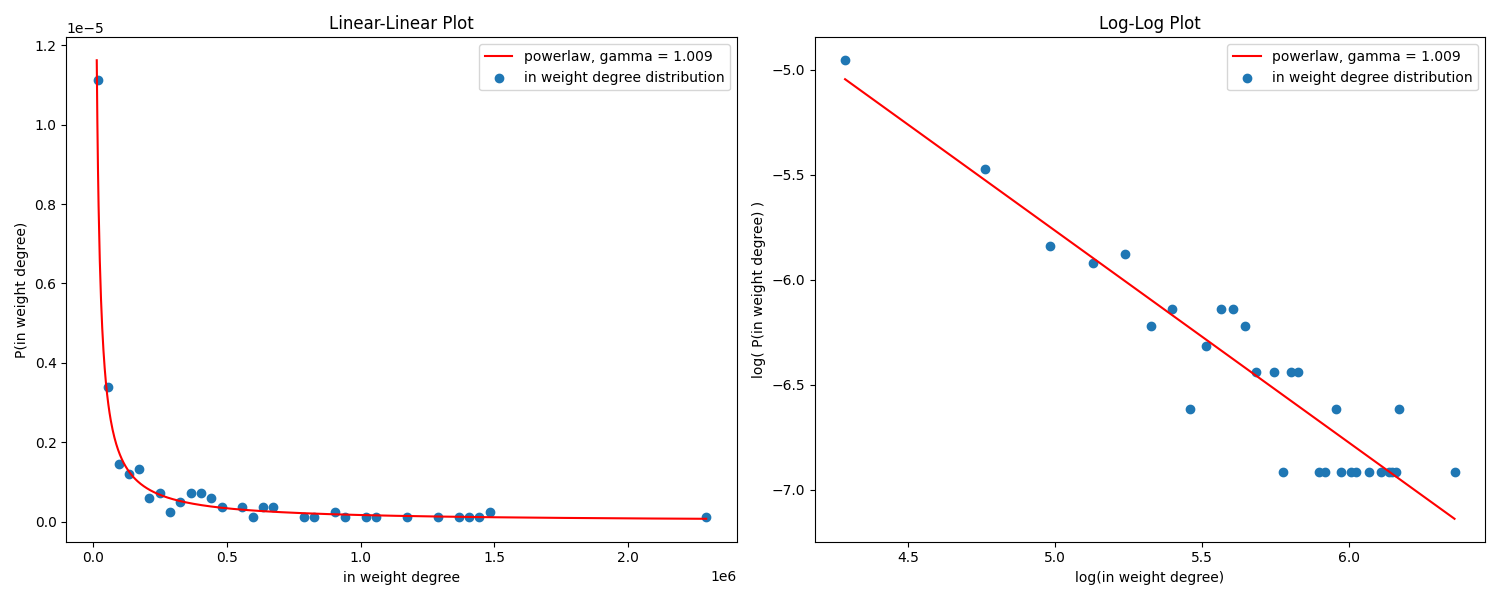
\includegraphics[width=\textwidth]{pics/powerlaw_in_weight_degree_p10_y2010.png}
    \caption{Food Products trade network's degree distribution of the \textit{in weighted degree} in 2010, with power law fit.}
    \label{fig:plfoodw}
\end{figure}

\subsubsection*{Network plot and node properties}

Let us also show the actual network in 2010 with nodes and edges, using the force-directed algorithm. The plot is shown in Figure \ref{fig:foodnetwork}. The first thing we notice here, thanks to the spring layout, is that the graph has a core-periphery structure. Most of the major economies are at the center of the graph, that is to say, they are the countries which are the top exporters of \textit{Food Products} to other nodes. We can identify them by considering the node size in the picture, which is proportional to the out weighted degree: a node is bigger if the corresponding country exports many goods of this category. At the center we find for example the European countries, which have a dense web of imports (the \textit{orange} exchanges) among themselves, and also a considerable number of exports to the peripheral countries (the \textit{pink} edges). Hence, the layout helps us identify which are the most central countries before looking at metrics: in the \textit{core} of the network we see nodes such as the Netherlands (NL), the United States (US), Germany (DE), Brazil (BR), France (FR), which have a high \textit{out degree}, with a high number of connections with peripheral nodes. If instead we were to look from the perspective of importing countries, we could identify which are the links of strongest dependence, intended here as the ones with the highest weight. These are shown in Table \ref{tab:top10foodimp}. In the top half, among the strongest dependencies, we find the exports from Denmark (DK) to Greenland (GL), from the United Kingdom (GB) to Falkland Island (FK) and from Spain (ES) to Andorra (AD). These are just few examples of territories politically linked to the primary country, and thus historically depending on it for the economy. The strongest incoming links for Italy (IT), instead, are reported in the bottom half of the table. We can observe that most of the countries that export the most \textit{Food Products} to IT are EU countries, and also that for this specific category the level of dependence is not as high as that of the ones in the top half of the table.


\begin{figure}
    \centering
    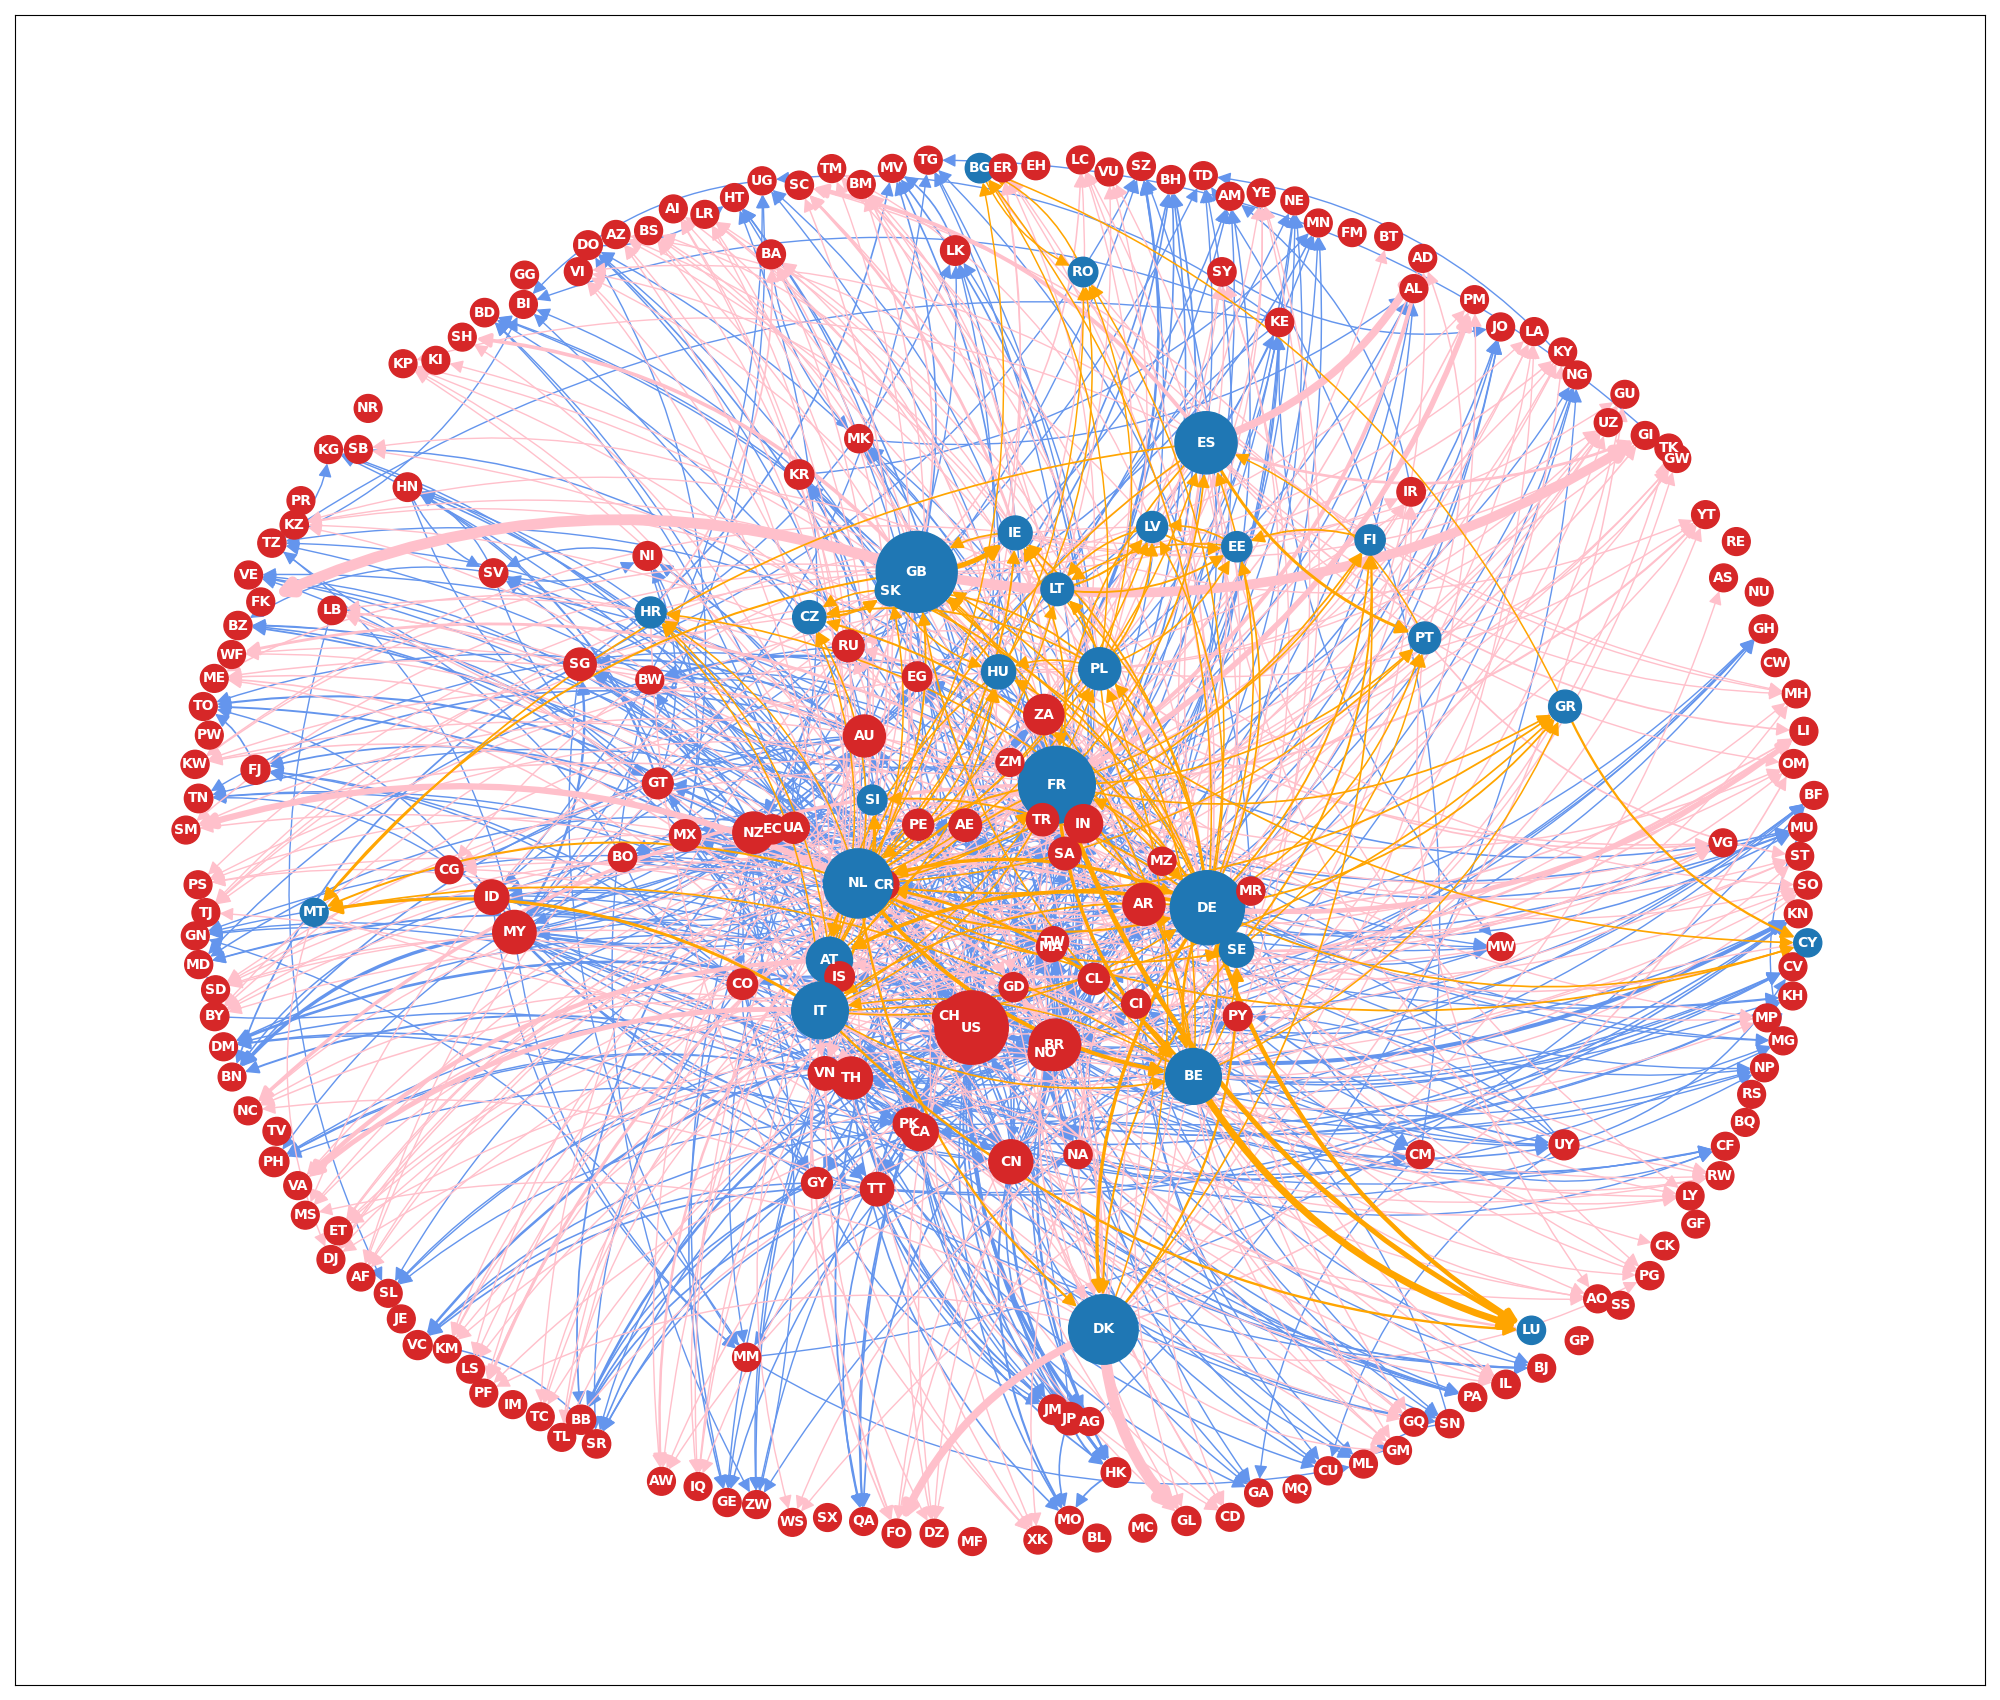
\includegraphics[width=0.8\textwidth]{pics/full_y10_p10_force_116.png}
    \caption[Global trade network of \textit{Food Products} in 2010.]{Global trade network of \textit{Food Products} in 2010. The size of the node represents the \textit{out-strength} of that country. The color of the node indicates EU countries (\textit{blue}) and non-EU (\textit{red}); the color of the edge is \textit{orange} for intra-EU exchanges, \textit{pink} for EU - non-EU exchanges and \textit{azure} for extra-EU exchanges. Only the top 5 import partnership for each country are shown.}
    \label{fig:foodnetwork}
\end{figure}

\begin{table}
    \centering
    \begin{tabular}{llr}
\toprule
Country From & Country To & Value €/1000 p. \\
\midrule
          DK &         GL &      1463214.81 \\
          GB &         FK &      1426621.59 \\
          GB &         GI &      1235017.11 \\
          ES &         AD &       953921.43 \\
          DK &         FO &       947595.33 \\
          BE &         LU &       836591.73 \\
          NL &         SM &       735949.98 \\
          FR &         PM &       623087.90 \\
          FR &         LU &       542263.65 \\
          GB &         IE &       536479.49 \\
\midrule
          DE &         IT &        69071.78 \\
          FR &         IT &        52386.18 \\
          ES &         IT &        43262.14 \\
          NL &         IT &        30148.72 \\
          BE &         IT &        14596.66 \\
          AR &         IT &        13405.36 \\
          AT &         IT &        12854.69 \\
          DK &         IT &        10292.91 \\
          PL &         IT &         8509.97 \\
          GB &         IT &         8066.08 \\
\bottomrule
\end{tabular}
    \caption{Top 10 edges by weight in the \textit{Food products} market and top 10 incoming edges for Italy (IT) by weight, in 2010.}
    \label{tab:top10foodimp}
\end{table}

Let's consider now a specific country and have a look in detail at its position in the network and over time. In Figure \ref{fig:nedmetrics}, I considered the Netherlands (NL) and showed the main node properties. What is surprising to see is that although NL was one of the main exporters of \textit{Food Products} in 2010, we learn from this plot that since then both its \textit{out degree} and \textit{out strength} have been going up even more, meaning that the country has intensified its exportation output [CITARE GOVERNO NL]. The high value of out degree is consistent with the low values of Page Rank and authority values: given how these metrics are defined, it was to be expected, since NL has a lot of out going edges. Furthermore, a consideration can be made about the values of Hub, Out Degree and Clustering Coefficient. Although NL had higher values of Hub in the early years, after 2007 it has remained stable at low levels. This seems in contradiction with the increase in out degree, since one would expect a node with many connections to be a hub. However, this phenomenon can be explained by the simultaneous decrease in clustering coefficient: in fact, if the acquired out going connections of NL are all pointing towards peripheral countries, which have no connections among them since they don't act as exporters, and also they have low authority value since they don't buy goods from many other hub countries, then the hub value of NL itself is justified to stay stable at low values.

\begin{figure}
    \centering
    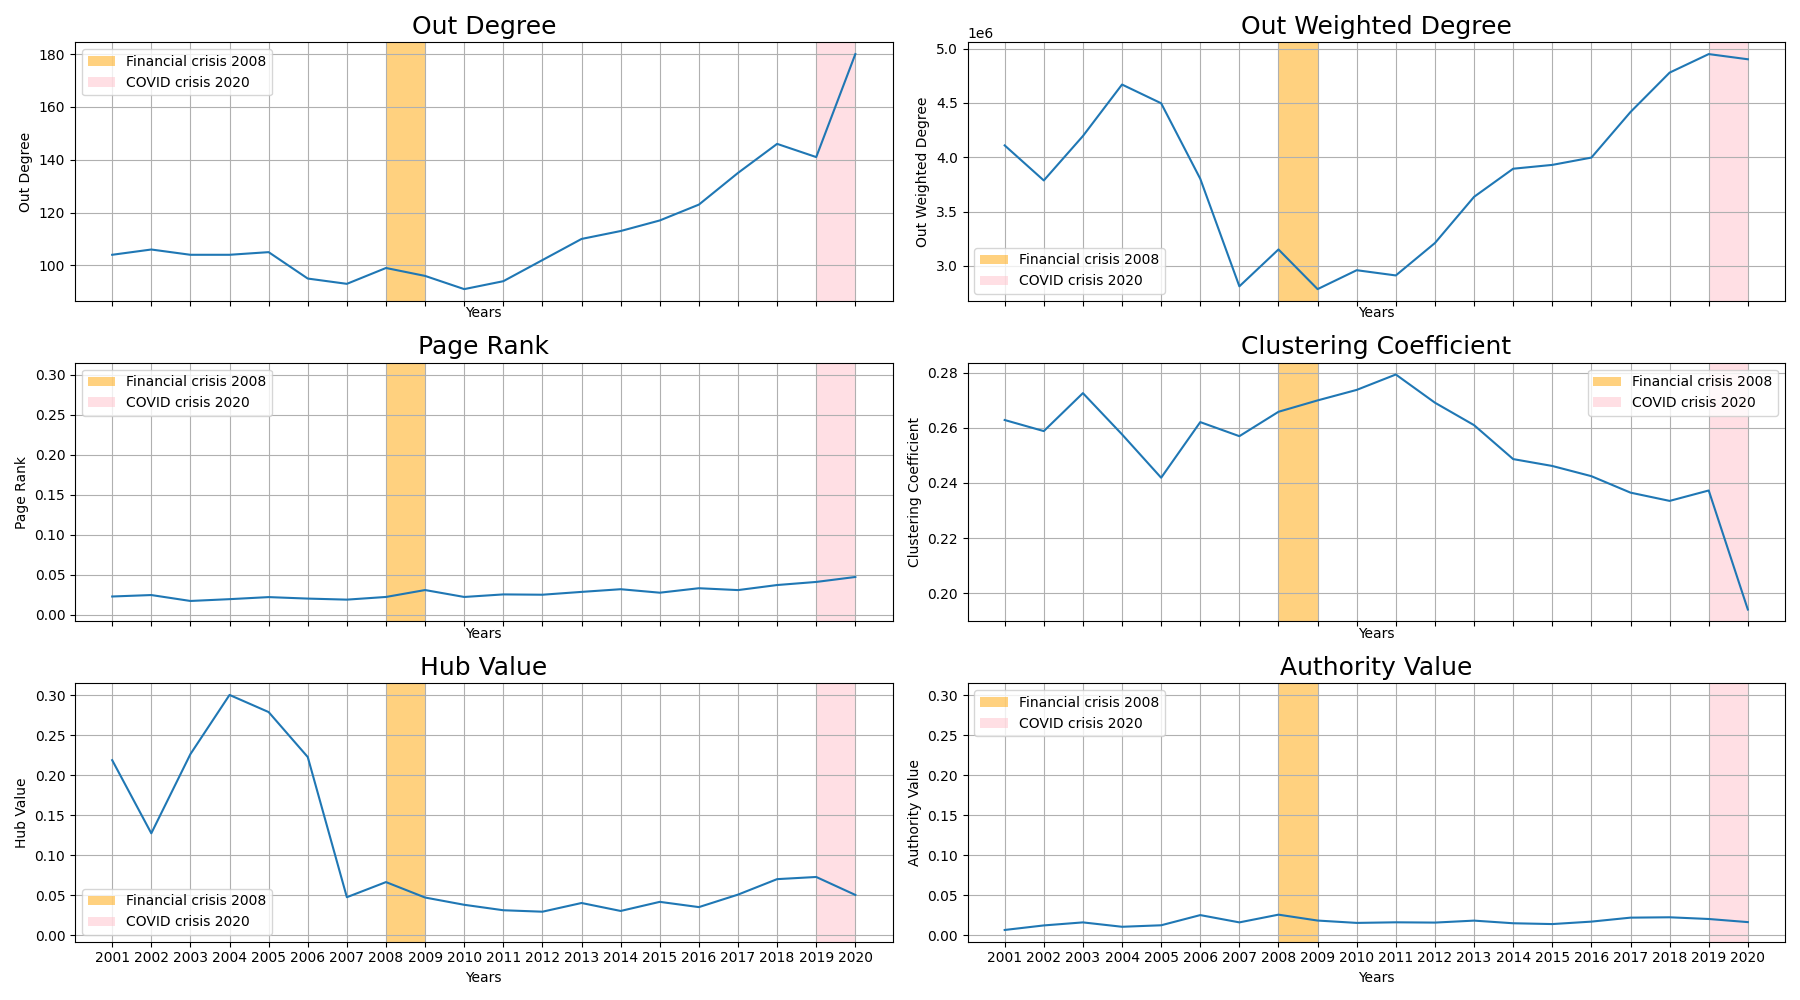
\includegraphics[width=\textwidth]{pics/NL_p10_metric_ts.png}
    \caption{Network metrics for the Netherlands (NL) of the trade market of \textit{Food Products} over the years.}
    \label{fig:nedmetrics}
\end{figure}

% \pagebreak
\subsubsection*{Community detection}

An alternative approach to study such trade networks is to understand their block structure. In recent years, this has been a hot topic in the research of network theory applied to real-life graphs. It was stated in previous chapters that the majority of these networks appear to have a \textit{core-periphery} structure, without however supporting the claim with any evidence. In this section, I will apply the methods of Degree Corrected Stochastic Block Model and Louvain Algorithm to the trade network of \textit{Food Products}. Analyzing the outputs of such algorithms can help us better understand the relationships among countries in this sector, and also verify whether the obtained clusters of countries support the idea of a core-periphery network. The two methods I used need to be fed slightly different networks: while for Louvain an extension of the modularity metric for weighted connections exists, for SBM and DCSBM I had to use a binary network, and hence I followed the procedure explained in Section \ref{sec:3binarygraphs}. I have run both algorithms on each available year of the \textit{Food Products} trade network, with the following parameter settings:
\begin{itemize}
    \item DCSBM: $alpha = 0.1$, which is the parameter of the Dirichlet distribution over the vector of probabilities of memberships;
    \item Louvain Method: $resolution = 0.5$, which is the $\gamma$ parameter in the modularity formula (Equation \ref{eq:3deltamod}).
\end{itemize}
Let us start to look at the results from Figure \ref{fig:dcfood}: we have represented here a \textit{parallel categories} plot, in which numbers represent the communities found by the DCSBM algorithm, and the colors refer to the memberships of 2019. We can observe here that the method has identified 9 blocks in 2019, some of which like 1, 2 and 7 are also quite numerous. The peculiarity of this plot is that it allows us to see where the nodes in each community come from, and if they often changed membership through the years. In particular, while clusters like 1 and 7 have been almost always consistent, we deduce that community 2 is the result of an aggregation of countries that used to belong to many other different communities in past years, and that only from 2017 on they started to get together in a single group. It is worth noting that none of these are formal communities, meaning that the model is agnostic of any trade agreements among groups of countries, as for example the European Union. The algorithm takes only into account all the links of nodes with each other, and tries to identify patterns of countries behaving in the same way or having tight relationships.
Aside from DCSBM algorithm, we can also run the Louvain Method on the graphs, which, contrary to SBM, is a technique created primarily for community detection. In this case, the results are shown in Figure \ref{fig:loufood}. The first thing that we notice here is that the number of communities identified is lower, just three in 2019. The reason for this has to be found in the completely different functioning of the two methods: in fact, while DCSBM searches for nodes with stochastic equivalence, and this may lead to an output with more blocks, Louvain optimizes the modularity metric, which favors bigger blocks given the resolution parameter of $0.5$. Next, we also observe that only the green community (2) has quite preserved itself through the years, while the members of the purple (1) and yellow (3) ones come from different older clusters which have been dismembered.


\begin{figure}
    \centering
    \begin{subfigure}{\textwidth}
        \centering
        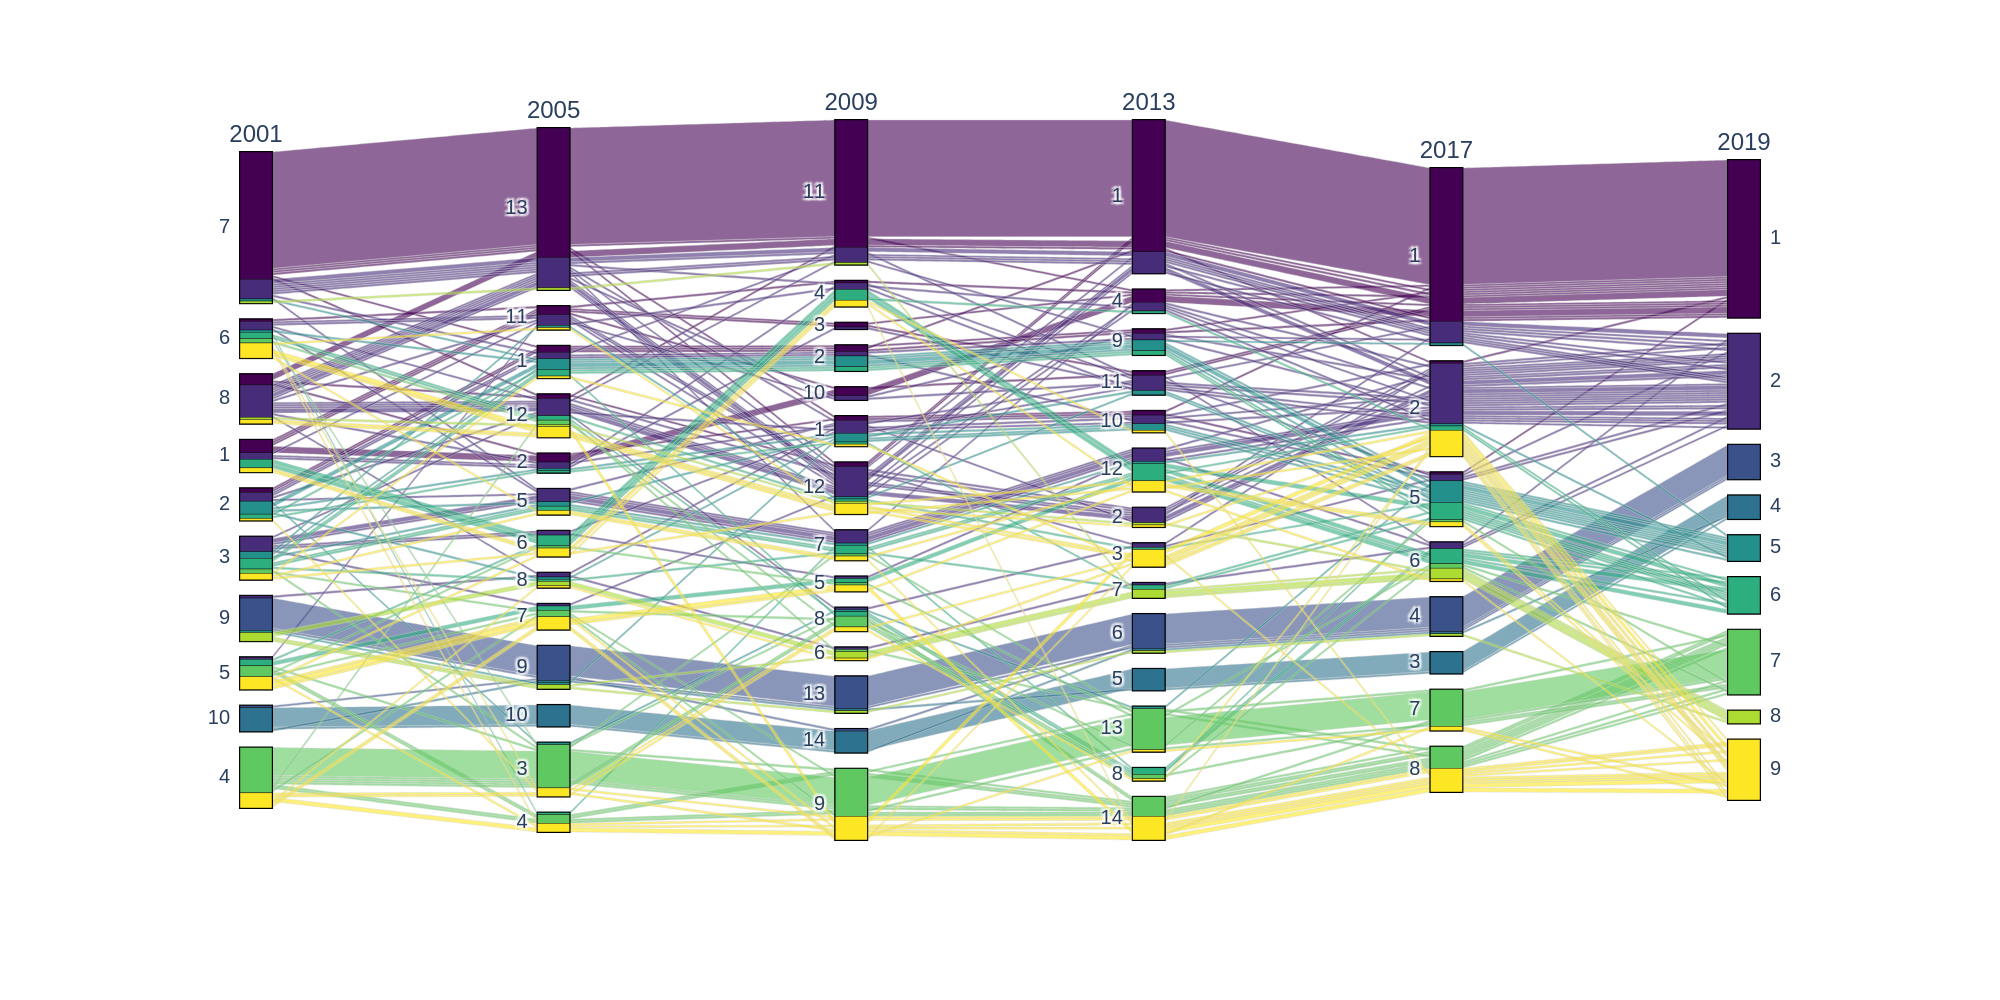
\includegraphics[width=\textwidth]{pics/dc_p10.png}
        \caption[Evolution over time of the communities of the \textit{Food Products} trade network, computed using the Degree Corrected SBM.]{Evolution over time of the communities of the \textit{Food Products} trade network, computed using the Degree Corrected SBM. Communities are shown every 4 years, plus 2019. The colors refer to the memberships in 2019.}
        \label{fig:dcfood}
    \end{subfigure}

    \begin{subfigure}{\textwidth}
        \centering
        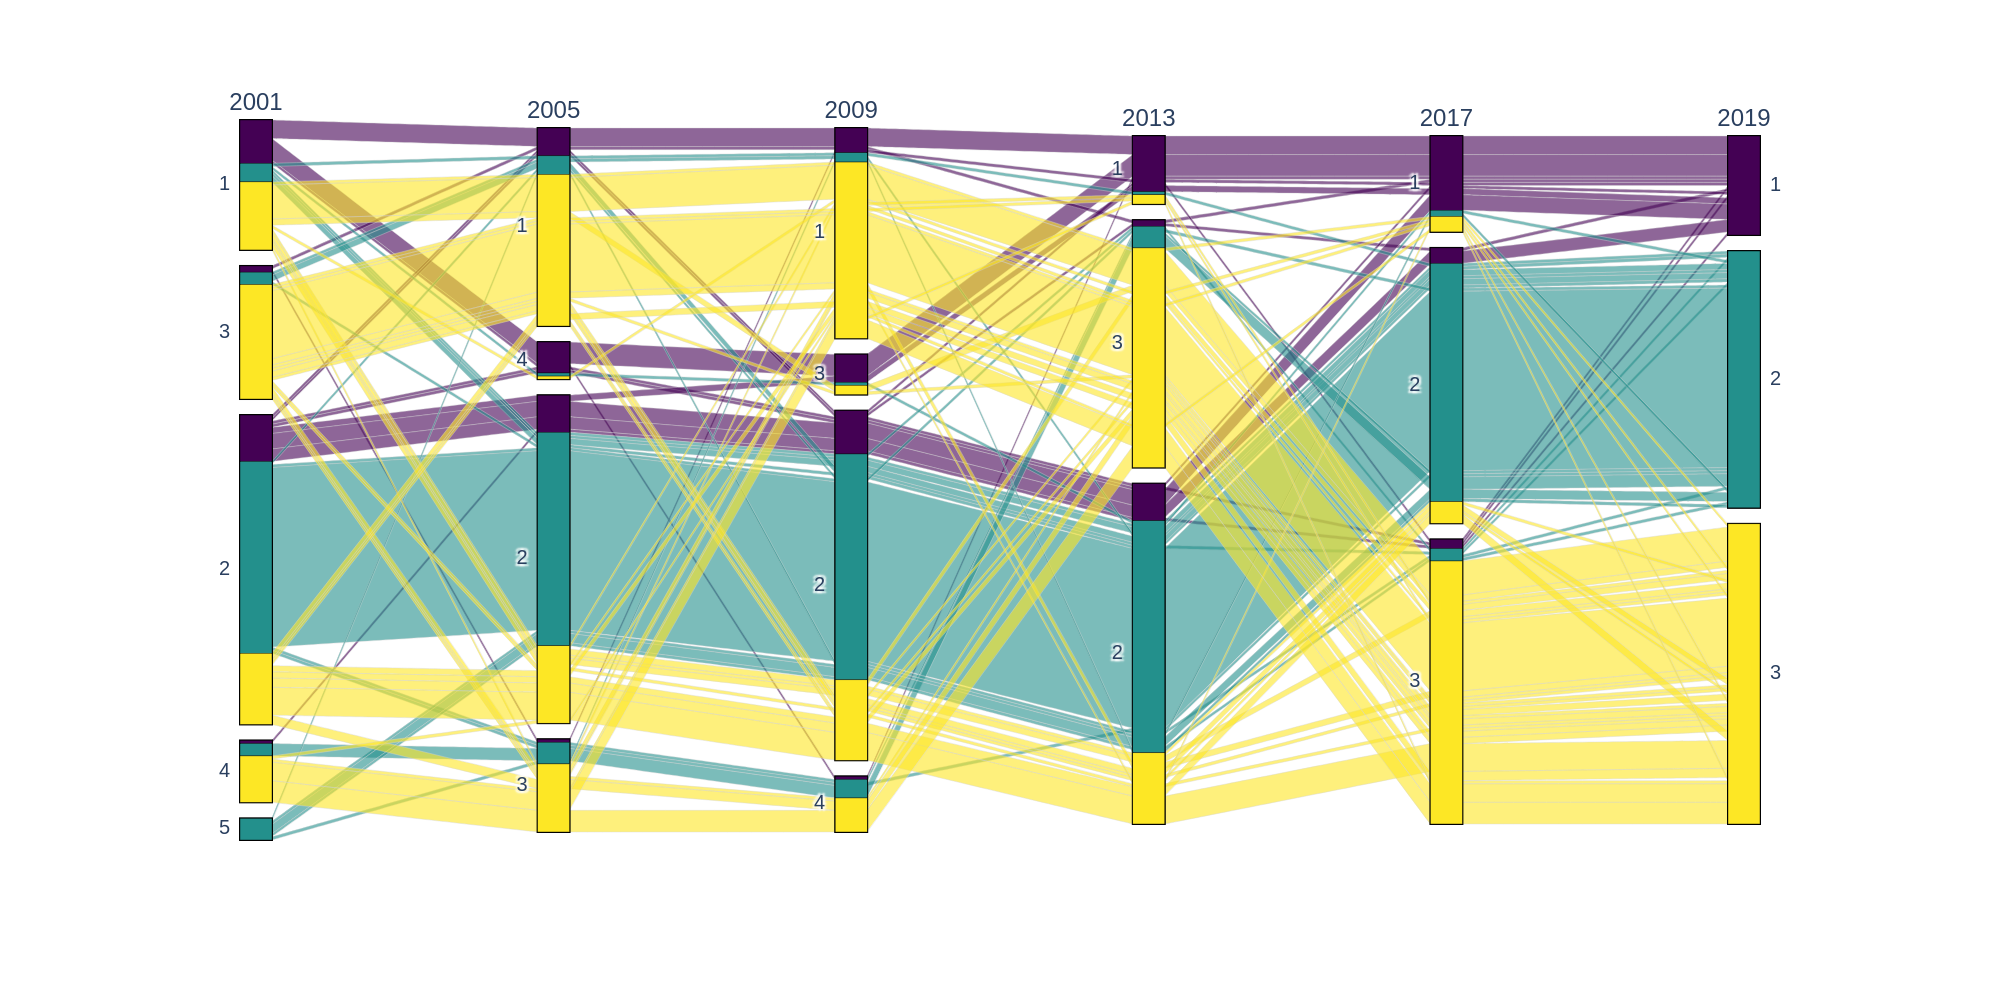
\includegraphics[width=\textwidth]{pics/lou_p10.png}
        \caption[Evolution over time of the communities of the \textit{Food Products} trade network, computed using the Louvain Method.]{Evolution over time of the communities of the \textit{Food Products} trade network, computed using the Louvain Method. Communities are shown every 4 years, plus 2019. The colors refer to the memberships in 2019.}
        \label{fig:loufood}
    \end{subfigure}
\end{figure}

The type of plots like in Figures \ref{fig:dcfood} and \ref{fig:loufood} are only useful to see the evolution of communities in time, and how they formed, but they don't provide us any insight into how these are actually structured. To visualize this, I have taken the membership output in 2019 of both DCSBM and Louvain, and plotted the same network twice, with the communities coded in the colors of the nodes. They are shown in Figure \ref{fig:foodnetworkdc} and \ref{fig:foodnetworklou}, respectively. Considering the first plot, we can say that the result of DCSBM has successfully identified a \textit{core-periphery} structure (the number corresponds to the clusters of Figure \ref{fig:dcfood}): in the middle, we find the blue (3), purple (2) and green (6) communities, which as their position in the spring layout suggests, as well as the size of their nodes, are the major exporters in these sectoral trade network. Moreover, an additional insight can be gained by this community result: if we look carefully at the nodes belonging to the blue (3) and purple (2) blocks, we can see that they are almost all countries of the EU. Their division also, is not without sense: in fact, the former community includes countries such as NL, FR, DE which are big world (and thus EU) exporters, while the latter includes those countries which still trade considerably with the EU and are members, but they don't export as much. The green community (6) of countries instead, could be defined as composed of mainly non-EU countries (like US, TH, NZ) but which are still relevant in the export market for \textit{Food Products}. A similar reasoning can be done for the plot below, where the communities of the Louvain method are displayed, but with a fundamental difference. While in DCSBM peripheral countries are more likely to belong to a community of their own, in Louvain they belong to the same community of the core countries with which they trade the most. In fact, we could say that light green countries (3) exchange highly with EU countries, while the dark green (2) ones trade mostly with non-EU countries. Furthermore, it can be noticed that both DCSBM and Louvain have captured the same community structure as to what it concerns the core exporting countries.

\begin{figure}[H]
    \centering
    \begin{subfigure}{0.8\textwidth}
        \centering
        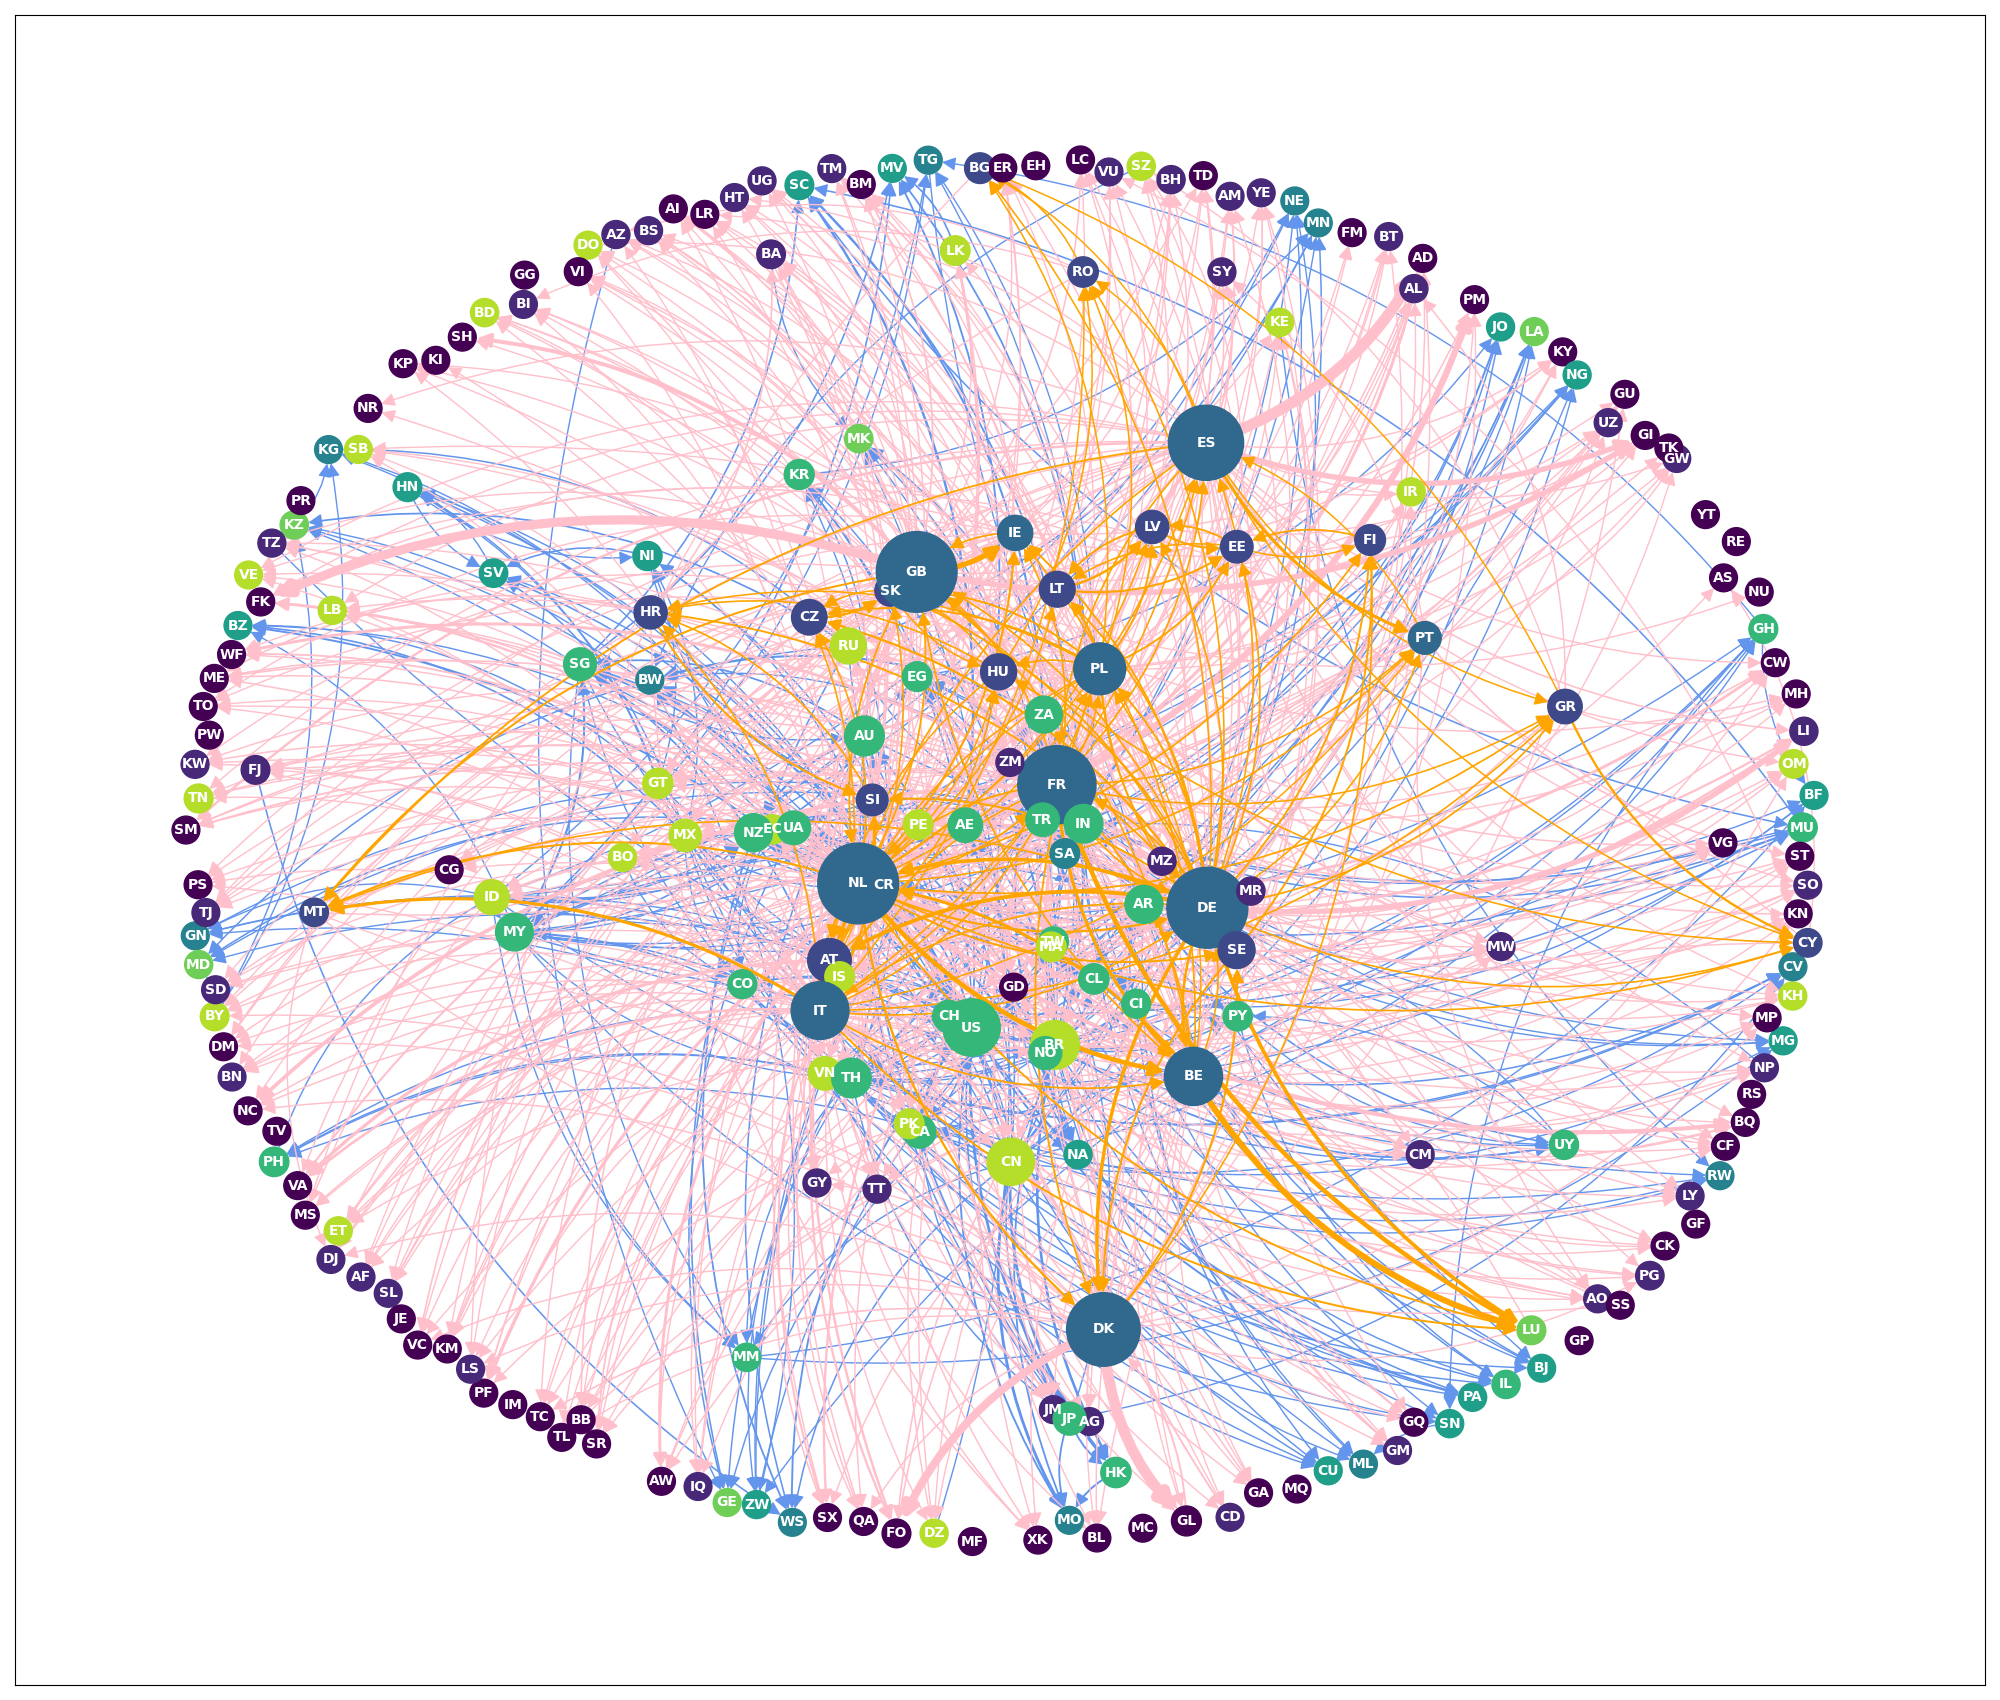
\includegraphics[width=\textwidth]{pics/full_y19_p10_force_143_dc.png}
        \caption{Degree Corrected SBM}
        \label{fig:foodnetworkdc}
    \end{subfigure}

    \begin{subfigure}{0.8\textwidth}
        \centering
        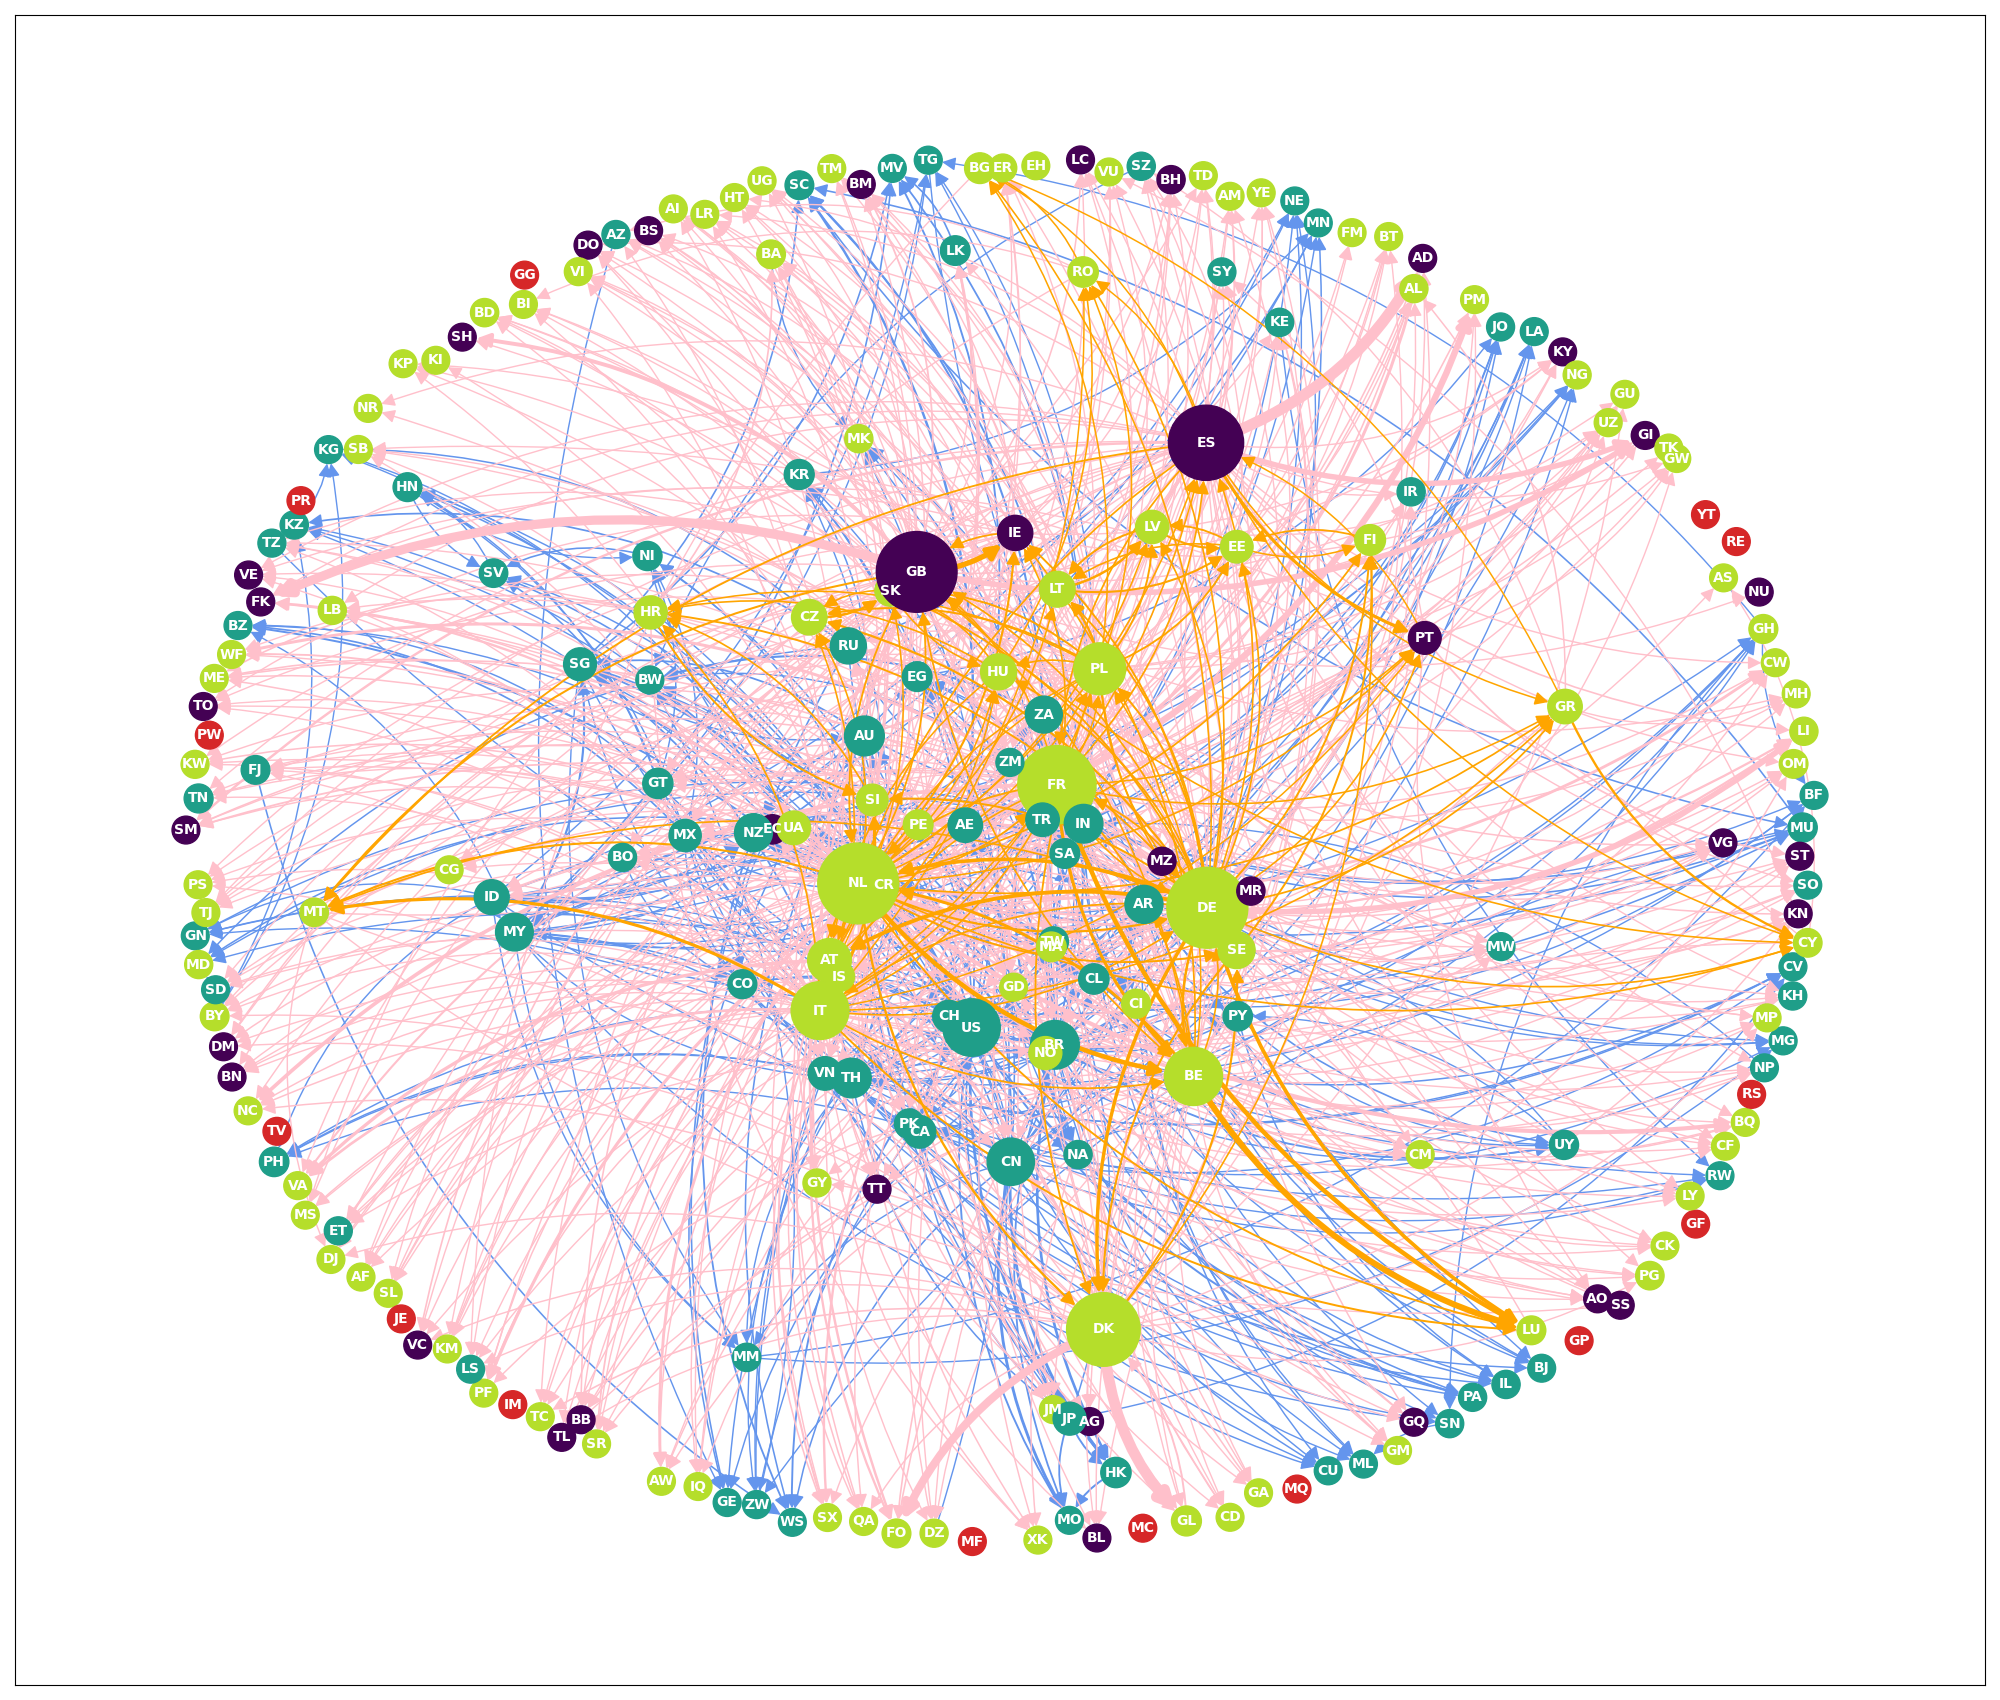
\includegraphics[width=\textwidth]{pics/full_y19_p10_force_144_lou.png}
        \caption{Louvain Method}
        \label{fig:foodnetworklou}
    \end{subfigure}
    \caption[Global trade network of \textit{Food Products} in 2019, with communities.]{Global trade network of \textit{Food Products} in 2019. The size of the node represents the \textit{out-strength} of that country. The color of the node corresponds to the block membership; the color of the edge is \textit{orange} for intra-EU exchanges, \textit{pink} for EU - non-EU exchanges and \textit{azure} for extra-EU exchanges. Only the top 5 import partnership for each country are shown.}
    \label{fig:foodcommunities}
\end{figure}